\documentclass[ngerman,hyperref={pdfpagelabels=false}]{beamer}

% -----------------------------------------------------------------------------

\graphicspath{{images/}}

% -----------------------------------------------------------------------------

\usetheme{KIT}

\setbeamercovered{transparent}
%\setbeamertemplate{enumerate items}[ball]

\newenvironment<>{KITtestblock}[2][]
{\begin{KITcolblock}<#1>{#2}{KITblack15}{KITblack50}}
{\end{KITcolblock}}

\usepackage[ngerman,english]{babel}
\usepackage[utf8]{inputenc}
\usepackage[TS1,T1]{fontenc}
\usepackage{array}
\usepackage{multicol}
\usepackage[absolute,overlay]{textpos}
\usepackage{beamerKITdefs}
\usepackage{caption}

\pdfpageattr {/Group << /S /Transparency /I true /CS /DeviceRGB>>}	%required to prevent color shifting withd transparent images


\title{Kolloquium Implementierungsphase RetroMachines}
\subtitle{Team B (RetroFactory)}

\author[Team B (RetroFactory)]{Team B (RetroFactory)}
\institute{Institut für Programmierparadigmen}

\TitleImage[width=\titleimagewd,height=\titleimageht]{titel}

\KITinstitute{Institut f\"ur Programmierparadigmen}
\KITfaculty{Fakult\"at f\"ur Informatik}

% -----------------------------------------------------------------------------

\begin{document}
\setlength\textheight{7cm} %required for correct vertical alignment, if [t] is not used as documentclass parameter


% title frame
\section{Deckblatt}
\begin{frame}
  \maketitle
\end{frame}

\section{Unser Projekt}
\begin{frame}
\frametitle{Unser Projekt - Wiederholung}
\begin{itemize}
\item Spielerische Darstellung des Lambda-Kalküls
\end{itemize}
\begin{figure}
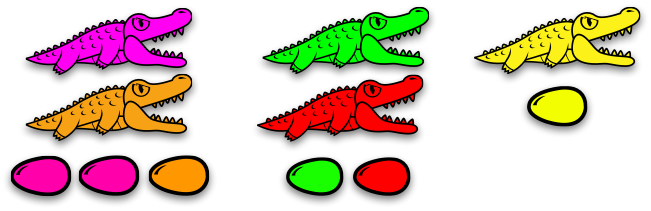
\includegraphics[width=0.5\textwidth]{AlligatorEggs.png}
\caption*{Ursprüngliche Spielidee von Bret Victor}
\end{figure}
\end{frame}

%Folie 2: Jump n Run statt Puzzle
\begin{frame}
\frametitle{Jump'n'Run statt Puzzle}
\begin{figure}
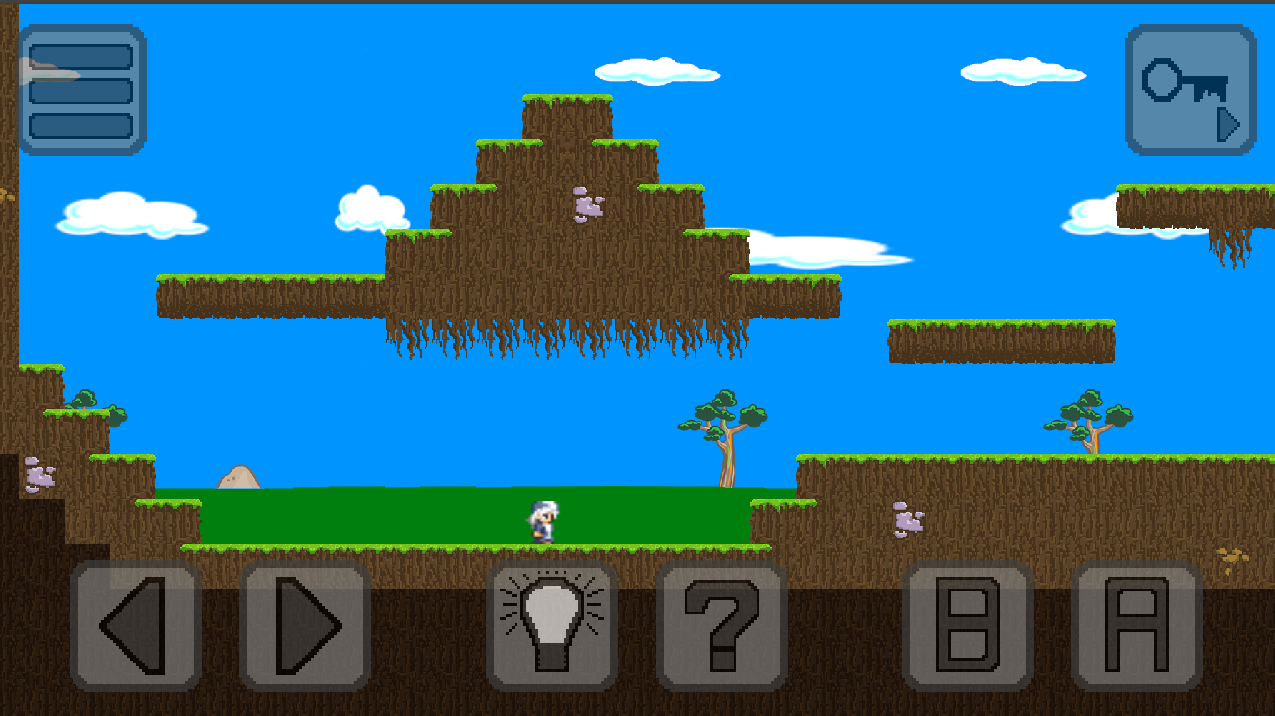
\includegraphics[scale=0.13]{RetroFactory.png}
\vfill
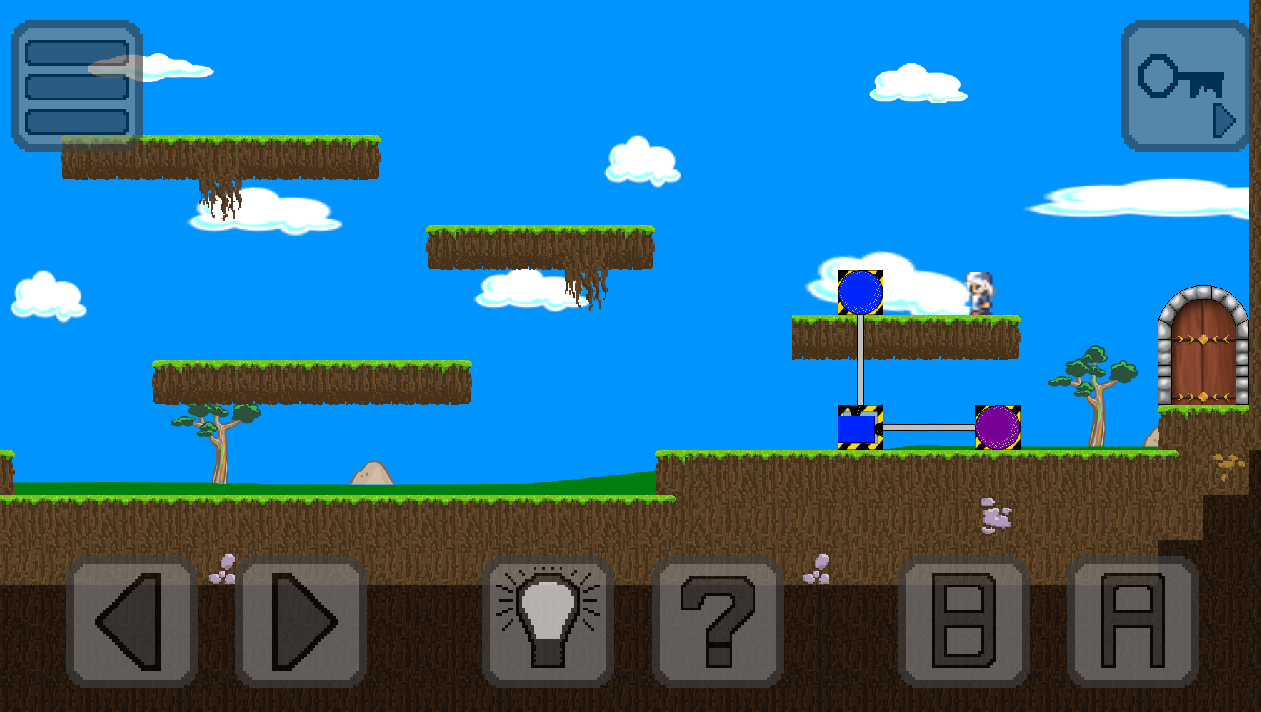
\includegraphics[scale=0.13]{ablagen.png}
\end{figure}
\end{frame}


\section{Änderungen am Entwurf}
\begin{frame}
	\frametitle{Änderungen am Entwurf}
	\begin{itemize}
	\item Lambda-Datenstruktur
	\begin{itemize}
	\item Subklassen statt enums
	\end{itemize}
	\item SQLite verworfen
	\begin{itemize}
	\item Verwaltung von LibGDX
	\end{itemize}
	\end{itemize}
\end{frame}

\section{Zeitplan}
\begin{frame}
	\frametitle{Zeitplan}
	\begin{center}
	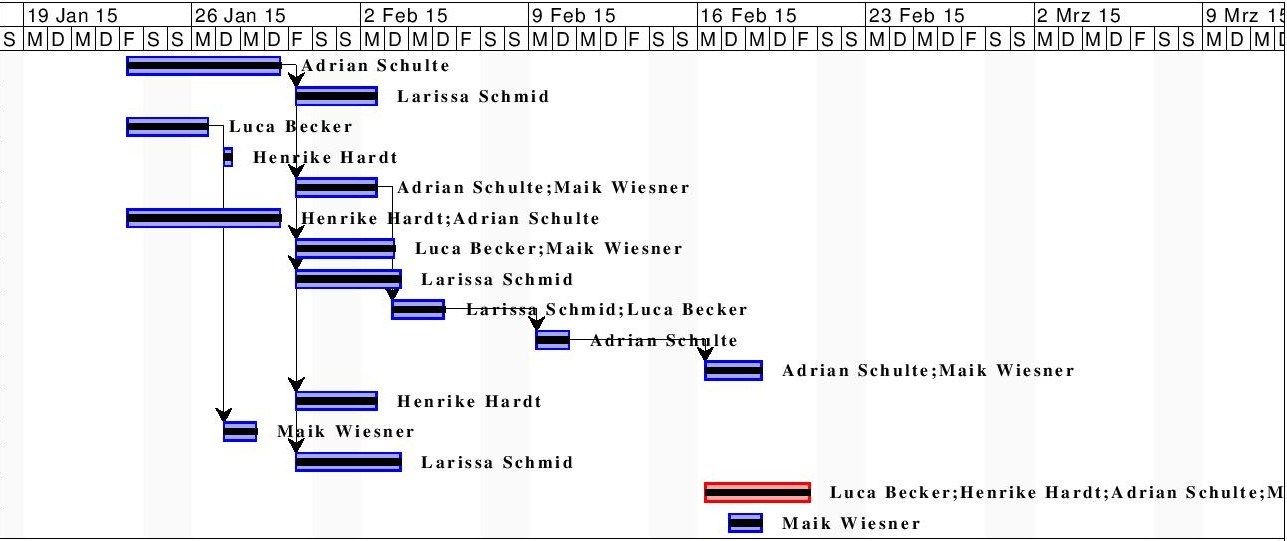
\includegraphics[width=\textwidth]{zeitplan_balken}
	\end{center}
\end{frame}

\section{Was wurde implementiert}
\begin{frame}
\frametitle{Was wurde implementiert\dots}
\begin{itemize}
\item alle Musskriterien
\item Folgende Wunschkriterien:
\begin{itemize}
\item Mehrere Spielcharaktere
\item Steuerung für Links- und Rechtshänder
\item Pixelgrafik / Retrolook
\end{itemize}
\end{itemize}
\end{frame}

\section{Statistik}
\begin{frame}
	\frametitle{Statistik}
	\includegraphics*[scale=0.2]{stats_timeline.png}
	\begin{itemize}
		\item LOC's: Java: 9713, Json: 986
		\item Anzahl Commits: 537
	\end{itemize}
\end{frame}

\section{Demo}
\begin{frame}
	\begin{center}
	\Huge
	\textbf{Live Demo!}
	\end{center}

\end{frame}

\end{document}
